\section{Implementation} \label{implementation}
Below are the different components that have been implemented to support this research. The entire implementation exists inside the Breda repository and is written in Rust and HLSL, this is why all code samples also use these languages.

\begin{wrapfigure}{r}{0.5\textwidth}
    \centering
    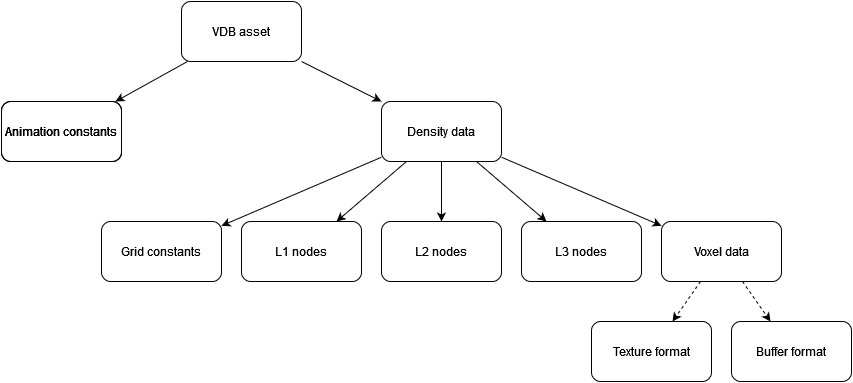
\includegraphics[width=\linewidth]{figures/vdb_asset.png}
    \caption{VDB asset data structure. Each VDB asset has constants for the entire animation, and density data. This density data has all the constants, nodes and voxel data. This voxel data can either be in buffer or texture layout. }
    \label{fig:vdb_asset}
\end{wrapfigure}

\subsection{Asset pipeline} \label{implementation:asset_pipeline}
The Breda asset pipeline is used to load all VDB files. This allows us to specify how our assets are loaded and processed, along with caching our final assets to reduce the amount of rebuilding. The main tweakable options for our VDB asset processing pipeline are the format, grid, filenames and clustering options. The format can be any of 32bit floating point, 16bit floating point, unsigned normalized (8bit float between 0 and 1) and BC7 \ref{related_work:texture_compression}. The grid specifies which grid in the VDB file we use as our density data. Usually, there are multiple grids in each VDB file, we can have density, temperature and volume type for example. All of these grids are used for different parts in a rendering pipeline, but for this research, we are only interested in a single grid and that is the density grid. The filenames option is used to select one or multiple VDB files, when entering multiple filenames we assume that these are an animation sequence. The clustering options consist of three things: (1) the number of clusters, which is $k$ when running k-means. (2) The number of iterations of k-means. And (3) the variance rejection threshold, which is used to specify how heterogeneous our bricks can be before we stop clustering them.

\begin{figure}[H]
    \centering
    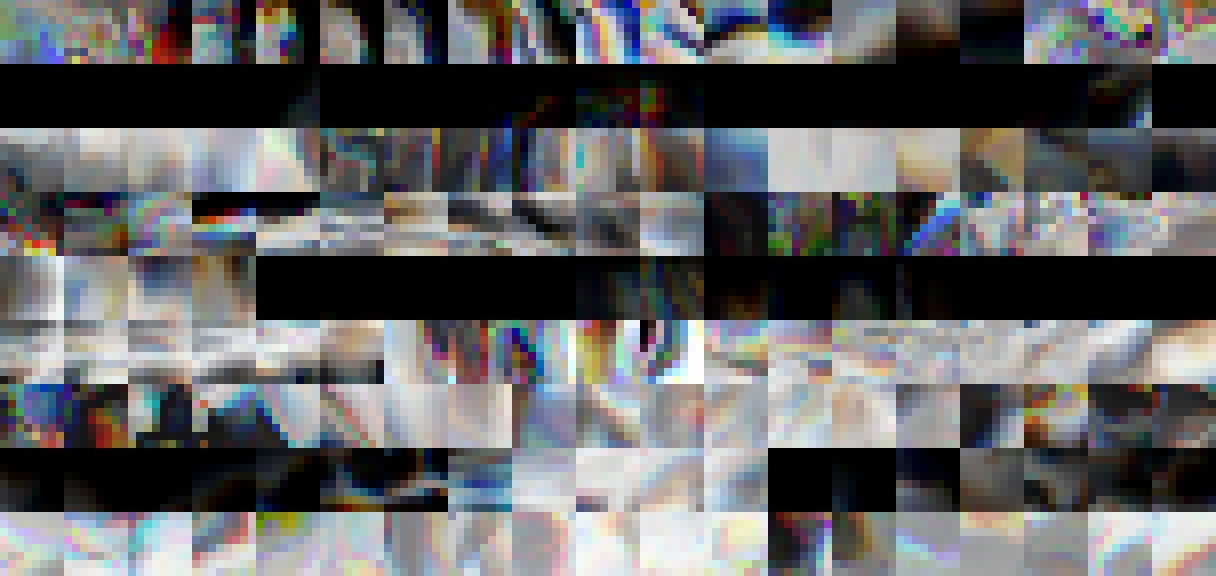
\includegraphics[width=\linewidth]{figures/voxel_memory_view.png}
    \caption{Voxel data texture captured by the Nsight frame debugger. Tiles of $8\times 8$ pixels can be seen. The third dimension, to get our brick data, is encoded using the RGBA color channels and the next texture slice. The tiles often contain gray values, meaning that the voxels in the z-axis are roughly the same (a pixel with roughly similar color values will always be a grayscale). However, some pixels are more colorful, which means that not all color channels are the same and there is either one voxel in the z-axis which is significantly different, or there is a gradient. This slice of the voxel brick data also showcases that even on this small scale of the individual brick level, there are many high-frequency details.}
    \label{fig:vdb_asset:memory_view}
\end{figure}


Using these options we can compute our VDB asset (The entire pipeline can be seen in Figure \ref{fig:vdb_asset_pipeline}). This consists mostly of constants and GPU-friendly vectors of data (see Figure \ref{fig:vdb_asset}). All nodes are implemented as structs which contain an unsigned integer to point to the next level of nodes and an array that contains unsigned integers. These are interpreted as the active child bit masks. In code, we refer to the internal nodes as L1, L2 and L3 nodes. L1 being the top level node with size $(1 << 5)^3$, L2 having size $(1 << 4)^3$ and L3 having size $(1 << 3)^3$ and pointing into the voxel data. The different animation frames are all unique L1 nodes. So if we want to render a specific frame we can simply take the frame ID and use that to index into the L1 nodes buffer, all pointers after that are handled at the asset creation stage. The full VDB asset creation process is listed below and with an overview in figure \ref{fig:vdb_asset_pipeline}.
\begin{enumerate}
    \itemsep0em
    \item First we read the metadata of our VDB files, which we then use to select which grid we want to read.
    \item Now we load the VDB data using vdb-rs \cite{VDBRS} which was developed during this research.
    \item Then we transform this data into our flat GPU-friendly data.
    \item The first pre-processing step consists of our deduplication scheme described in Section \ref{approach:clustering_similar_nodes}.
    \item After this we transform our data layout from our easy (and locally coherent) buffer layout to the texture layout.
    \item Then, depending on which format options were used, we compress our data. So we reduce our floating point data to either 16bit, 8bit or Bc7 texture data.
    \item After which we upload everything to the GPU.
\end{enumerate}

\begin{figure}[H]
    \centering
    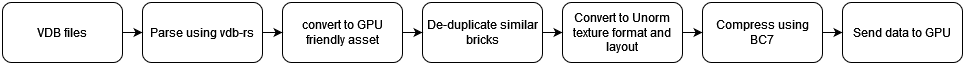
\includegraphics[width=0.9\linewidth]{figures/VDB asset pipeline.png}
    \caption{An overview of the asset creation pipeline.}
    \label{fig:vdb_asset_pipeline}
\end{figure}


\subsection{Shaders} \label{implementation:shaders}
To integrate the built data structure into Breda, two shaders have been written, \textit{VDB.hsls} and \textit{HDDA.hlsl}. The main way to interface with the data structure is contained in \textit{VDB.hlsl} which has functionality for getting voxels, getting the activity status of certain voxels, and checking what the deepest level of the tree a certain voxel is part of. \textit{HDDA.hlsl} is largely the same as implemented by \cite{museth2013vdb}. The main difference is that we make use of callbacks on the GPU, which is done by passing a template argument to the traversal function. This template argument must implement \textit{empty} and \textit{operator()} which are called after every step, or compiled away if either of them is not used. These step functions are used to write clean yet fast traversal code (as seen in Figure \ref{implementation:hdda_sample}).


\begin{figure}
    \begin{lstlisting}
    // The hdda march method has the following function signature
    // We explicitly say which level of our tree we want to traverse
    template <typename VoxelData, typename VoxelFn>
    void march(inout VoxelFn fn, Layer callbackLayer);

    // We define a struct that contains our traversal payload
    struct FirstDensityFn {
        float4 color;
    
        bool operator()(float voxelData, float t0, float t1, uint dataIndex) {
            float chunkIndex = voxelData * 360;
            color = float4(hsvToRgb(chunkIndex, 1, 1), 1);
            return false; // we do not want to continue traversal
        }
        bool empty(float t0, float t1, uint dataIndex) { 
            return true; // we continue traversal
        }
    };

    // Now we can simply perform our HDDA traversal as follows
    float4 traverseVolume(){
        Hdda hdda = Hdda::new_(volumeGrid, ray, inverseRay);
        FirstDensityFn fn;
        fn.color = float4(0,0,0,0);
        hdda.march<float>(fn, LayerVoxels); 
        return fn.color;
    }
\end{lstlisting}
    \caption{Simplified outline of the HDDA api.}\label{implementation:hdda_sample}
\end{figure}


\subsection{Compression} \label{implementation:compression}
As said in Sections \ref{approach:texture_compression} and \ref{approach:clustering_similar_nodes}, there are two types of compression of the voxel data going on. First, we will have a look at how to cluster similar bricks. This is largely done by using NDarray \cite{NDarray} for different linear algebra methods. The clustering process is divided up into the following steps:

\begin{enumerate}
    \itemsep0em
    \item We parse our voxel data into a 2D matrix where every brick is one row, allowing us to use per-row clustering algorithms.
    \item Then we calculate the variance of the density data of each brick and divide that by the brick's mean density to get a normalized variance.
    \item We reject the brick if the normalized variance is higher than our set threshold. This way we only keep bricks that have low variance and thus have a low likelihood of containing unique features (see Section \ref{approach:clustering_similar_nodes} for the reasoning behind this step).
    \item After which we run k-means on all low variance bricks, with a given $k$ and the number of iterations. Unfortunately, this can be an expansive step as k-means has an algorithmic complexity of $O(nk)$ where n is the number of bricks in this case, and $k$ is the number of requested new bricks. So when both are large this step will become unpractical. However, most of the low variance bricks can be represented by a few new bricks, so $k$ should not be large anyway.
    \item After we have a new set of bricks we just have to fix the pointers of our L3 nodes and merge the filtered high variance bricks with the new bricks, and we are done.
    \item In figure \ref{fig:implementation:compression:cluster} we see the results of this compression technique.
\end{enumerate}


\noindent Texture block compression is done after rearranging the data from a buffer layout to a texture layout. With this data layout we can reduce the floating point precision, or even use the existing intel texture compressor \cite{ISPCTextureCompressor} to encode our data into Bc7. After doing this we still have to tell our backend what the format is of our texture, and then we are done. We can reuse our HLSL code for all formats because HLSL automatically samples different floating point types correctly.




\subsection{VDB viewer} \label{implementation:vdb_viewer}
A prototyping application was created for visualizing VDB files. This application can be used to load a single VDB file and display multiple debug views of the model as can be seen in Figure \ref{implementation:vdb_viewer:debug_views}. This application also allows quick testing of compression schemes as it bypasses the standard asset pipeline system that was discussed in Section \ref{implementation:asset_pipeline}.

\begin{figure}[H]
    \centering
    \subfloat[Shaded by accumulating density along the primary ray. The body of the cloud is hollow as can be seen.]{
        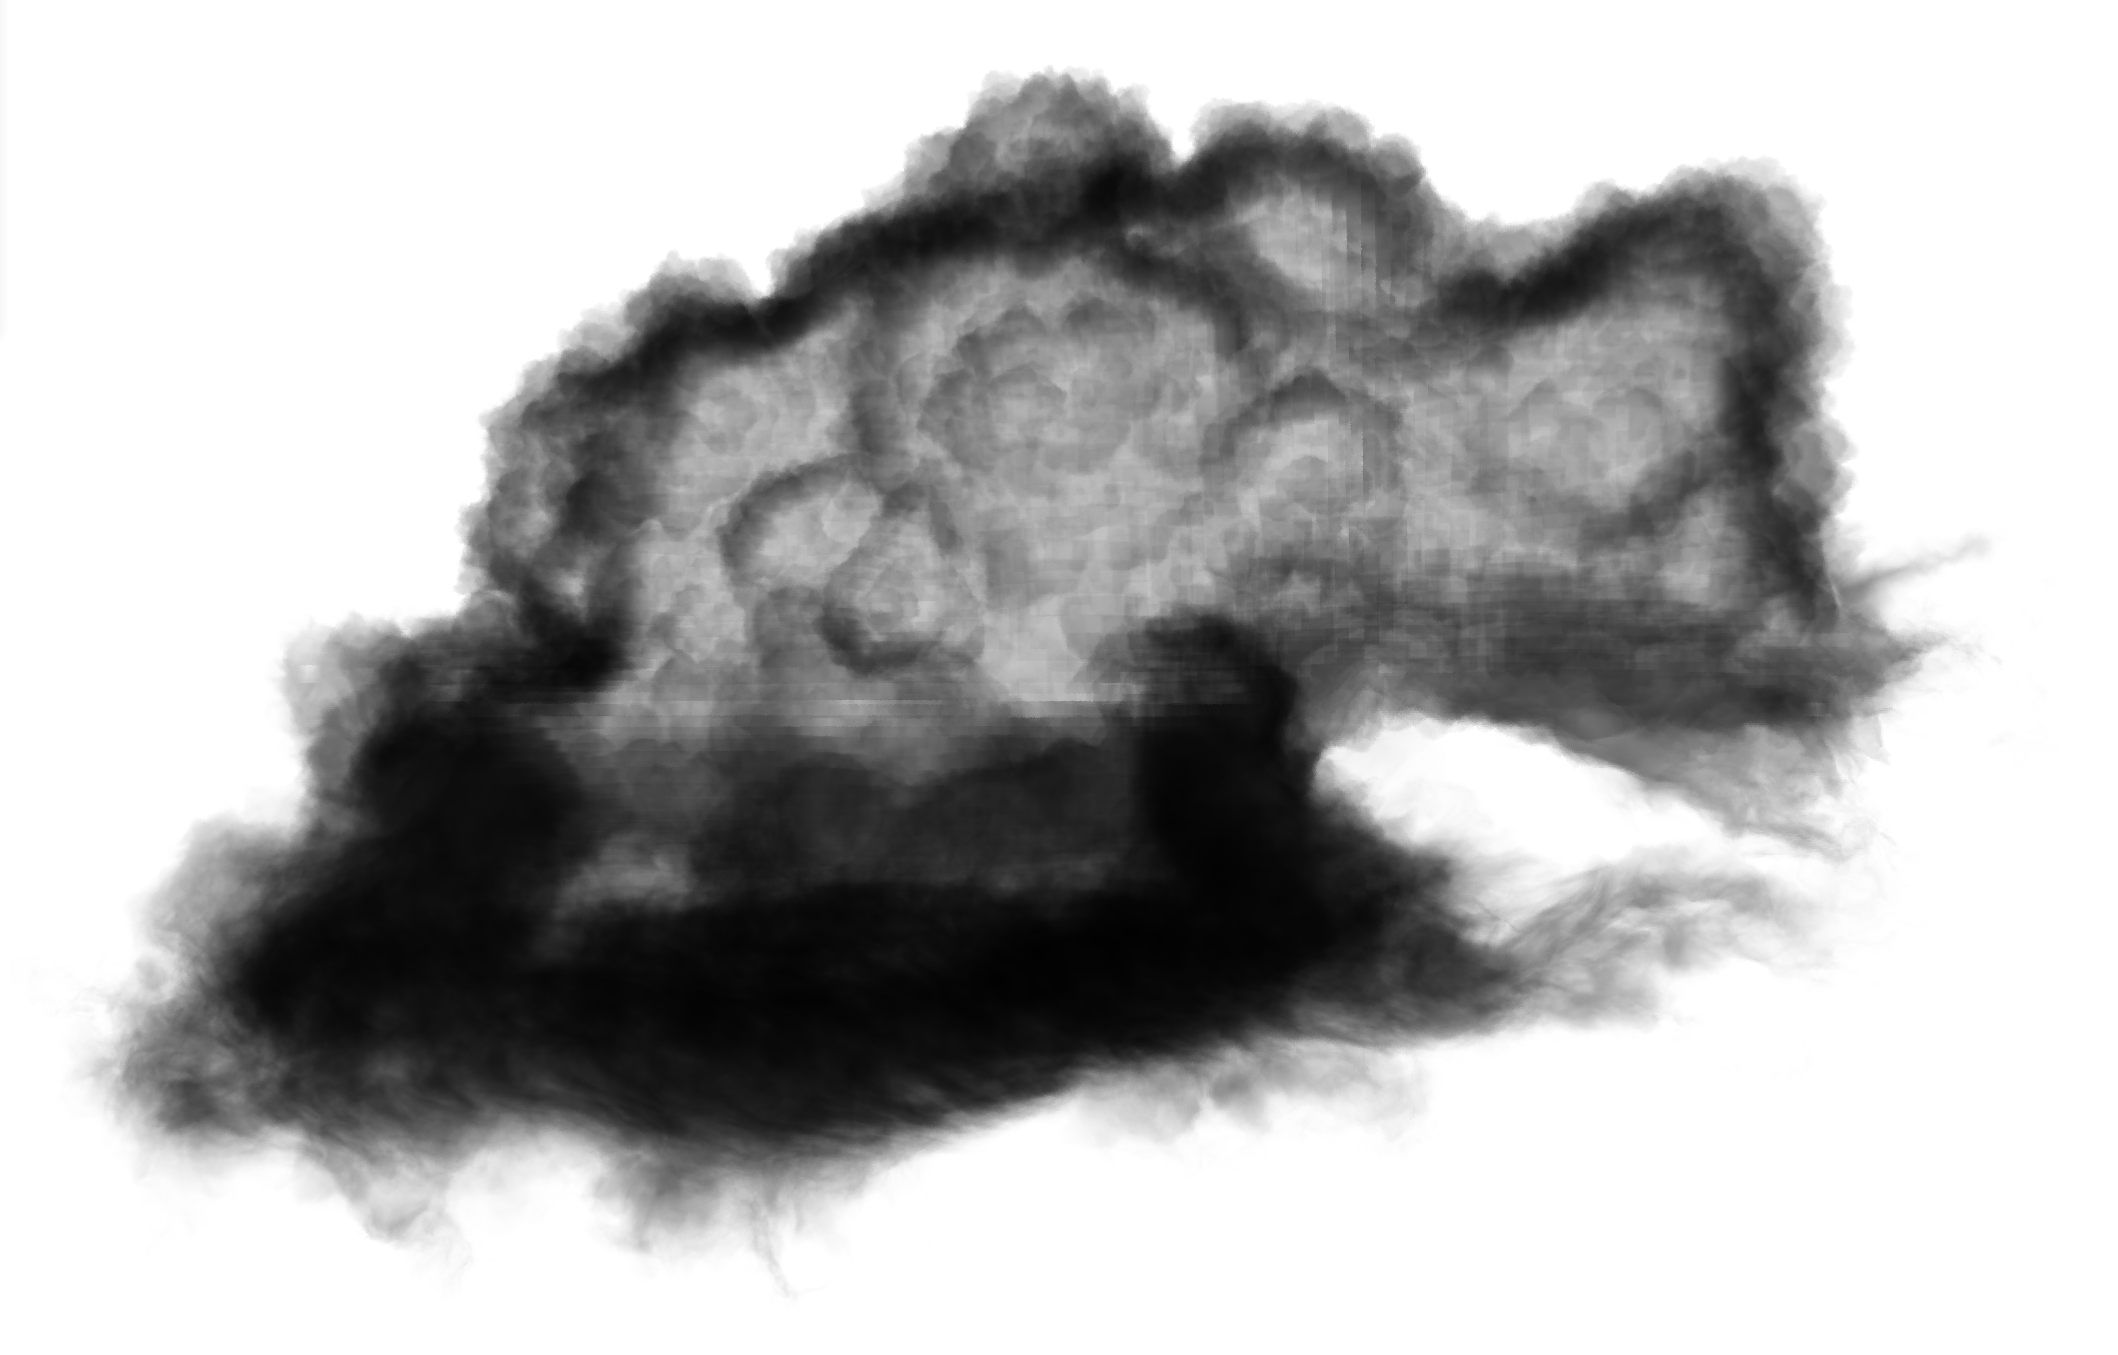
\includegraphics[width=0.45\textwidth]{figures/disney_cloud_half_res_shaded.png}
    }
    \hfill
    \subfloat[Shaded by depth of first hit voxel.]{
        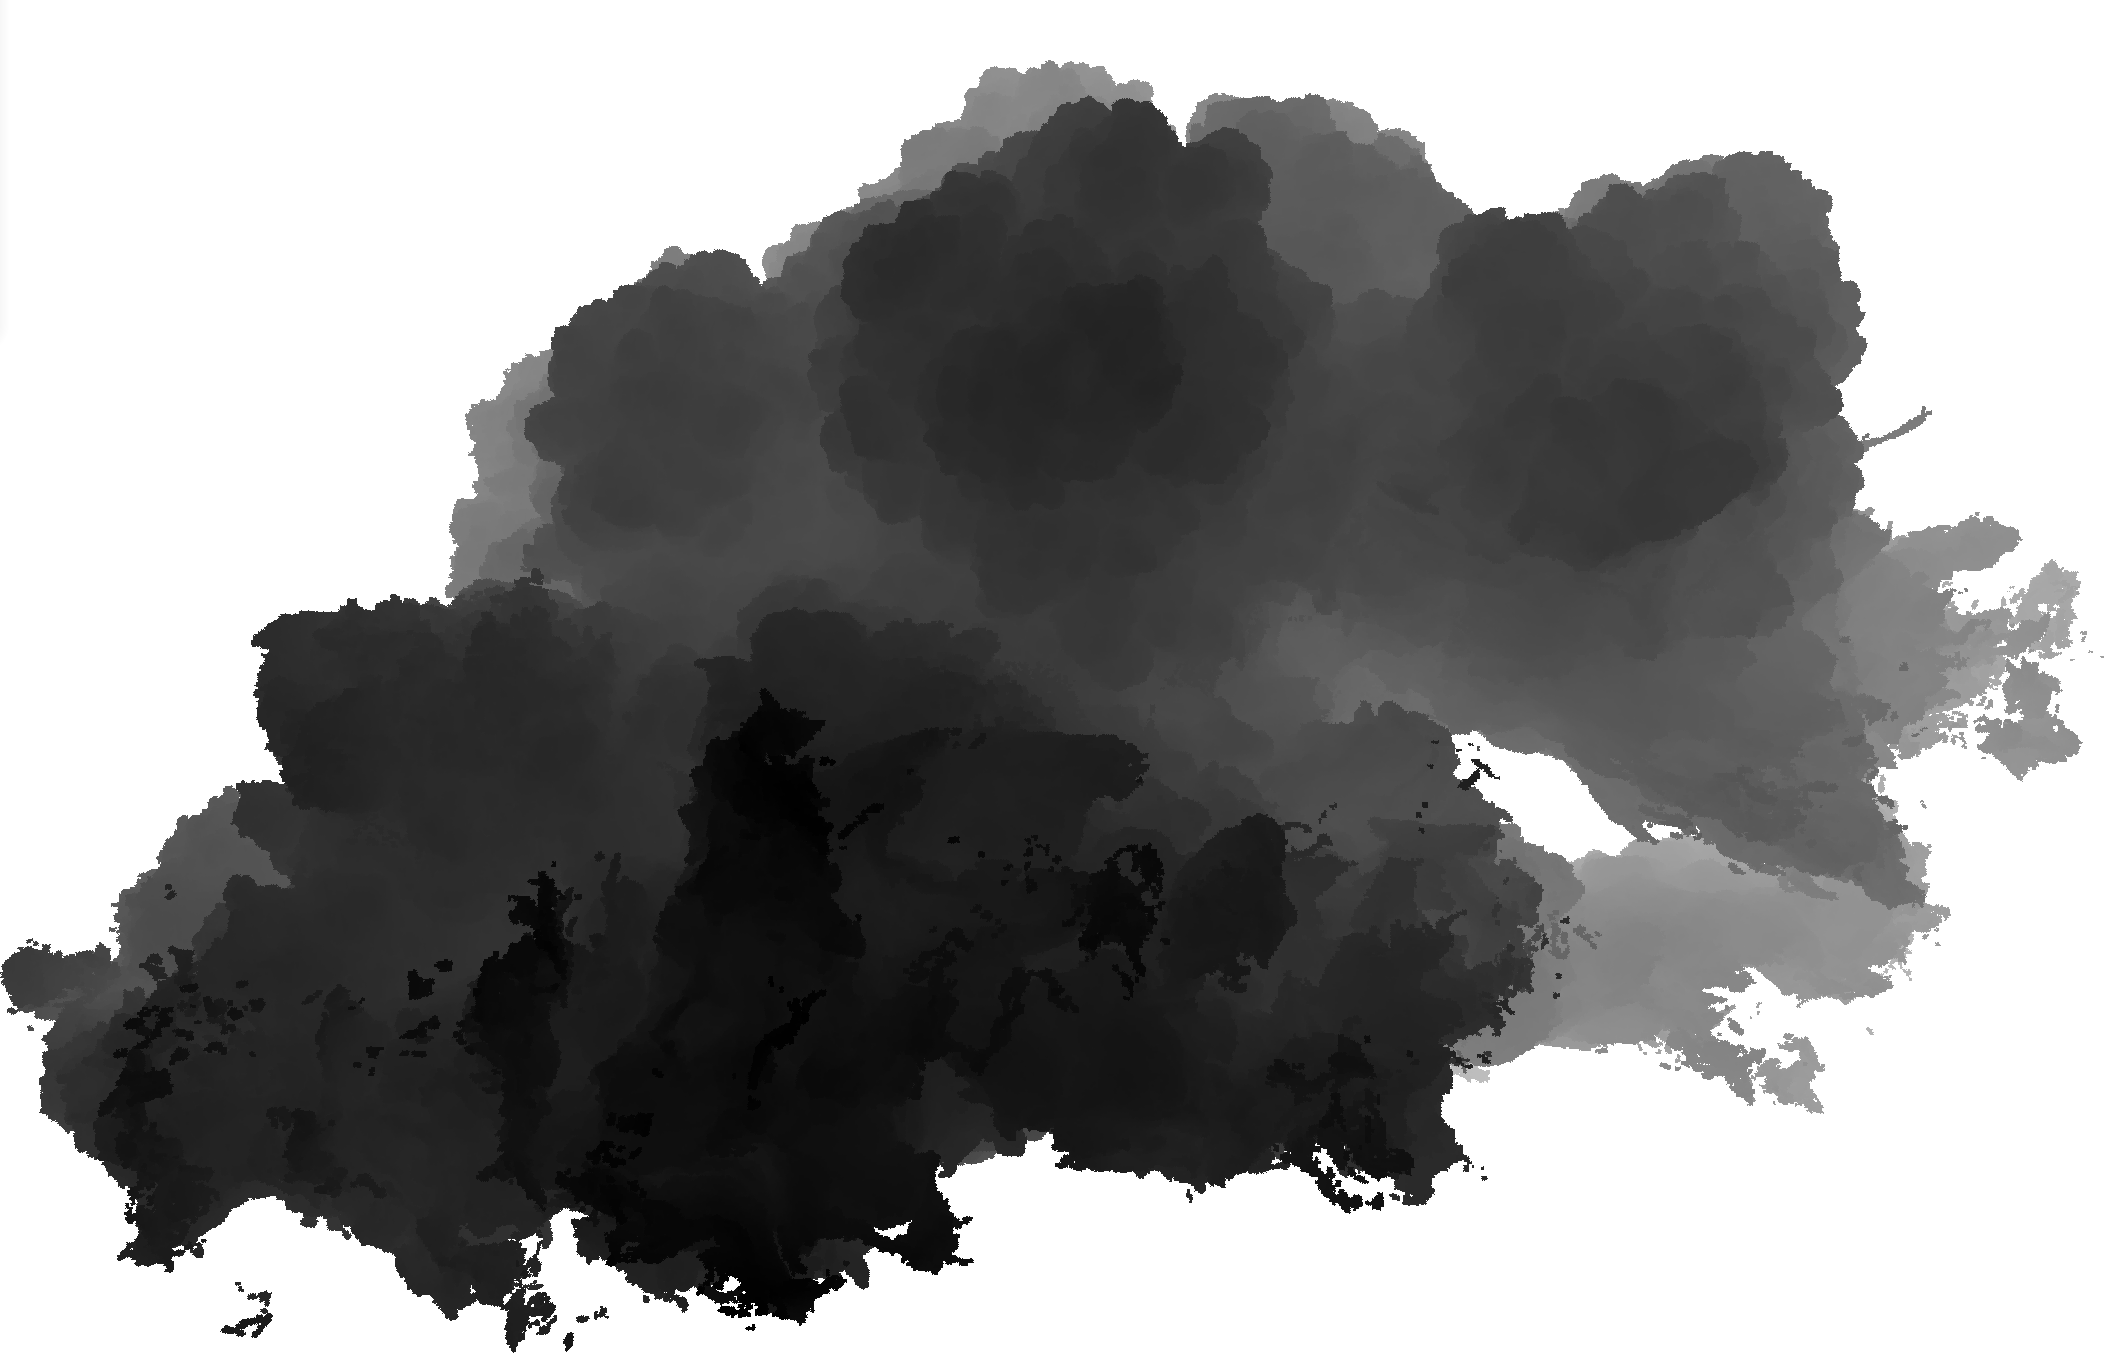
\includegraphics[width=0.45\textwidth]{figures/disney_cloud_half_res_depth.png}
    }
    \hfill
    \subfloat[Shaded by index into the voxel index. Shown is a conversion from index to hue using the following formula: $x + y\times dim\_size + z\times dim\_size^2$. The striped pattern is a result of bricks ($8^3$ voxels) are a combination of two texture slices, these are the altering index colors. The larger shifts in color, which are in specific cubic regions, correlate to the different L2 nodes.]{
        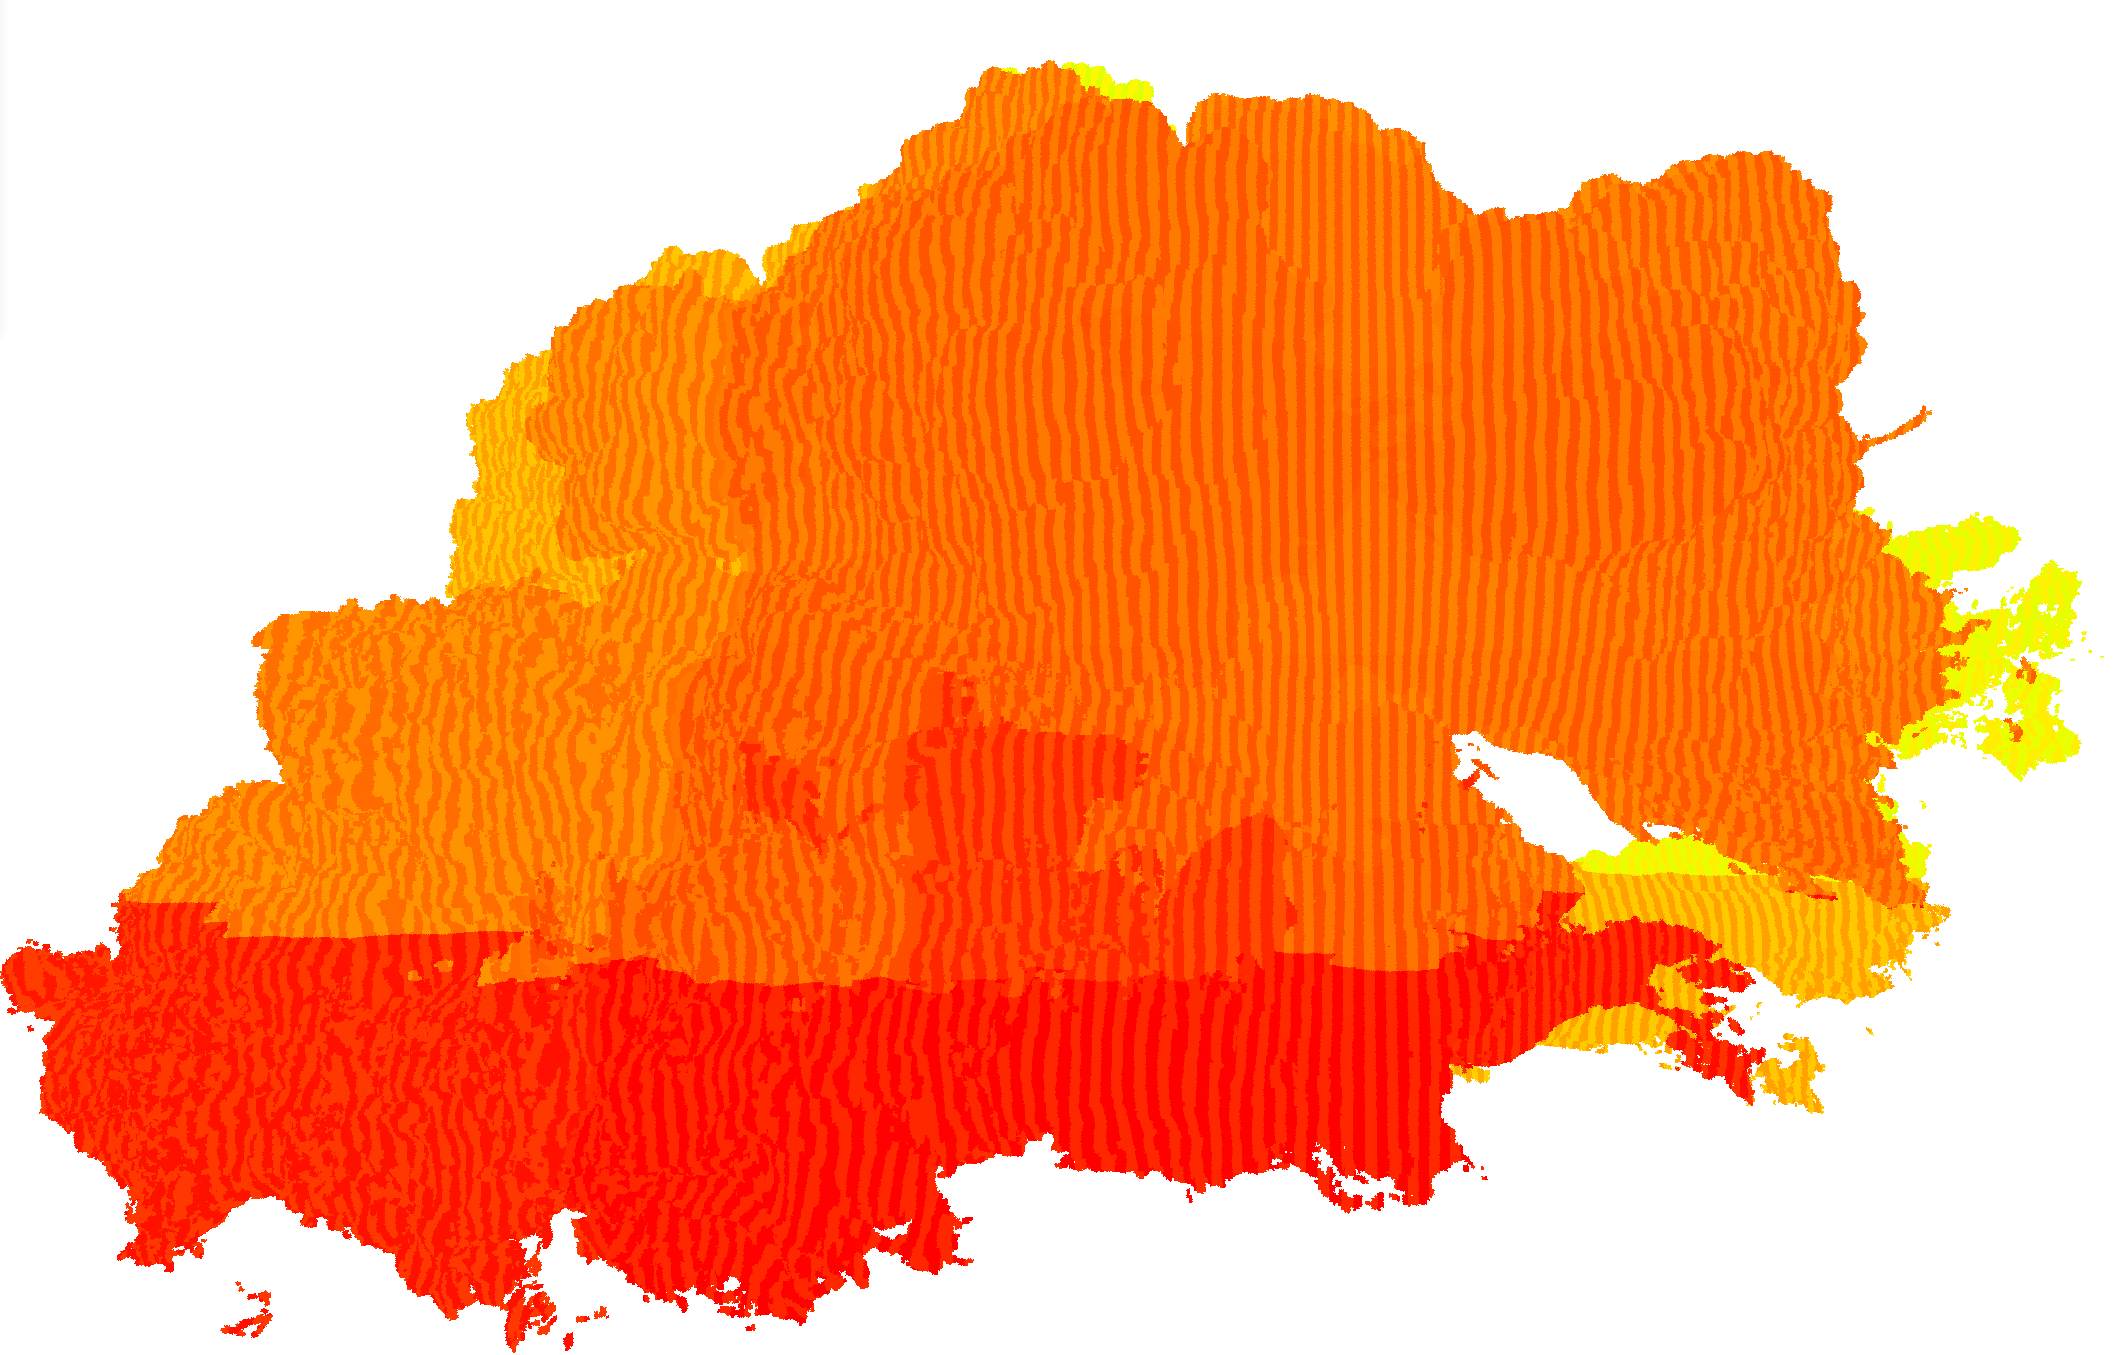
\includegraphics[width=0.45\textwidth]{figures/disney_cloud_half_res_index.png}
    }
    \hfill
    \subfloat[Shaded by the density of the first hit voxel, where a low density is red and a high density results in different hues. Overall the entire outside edge of the cloud only shows low-density voxels, but there are some spots where deeper voxels are visible which have a higher density.]{
        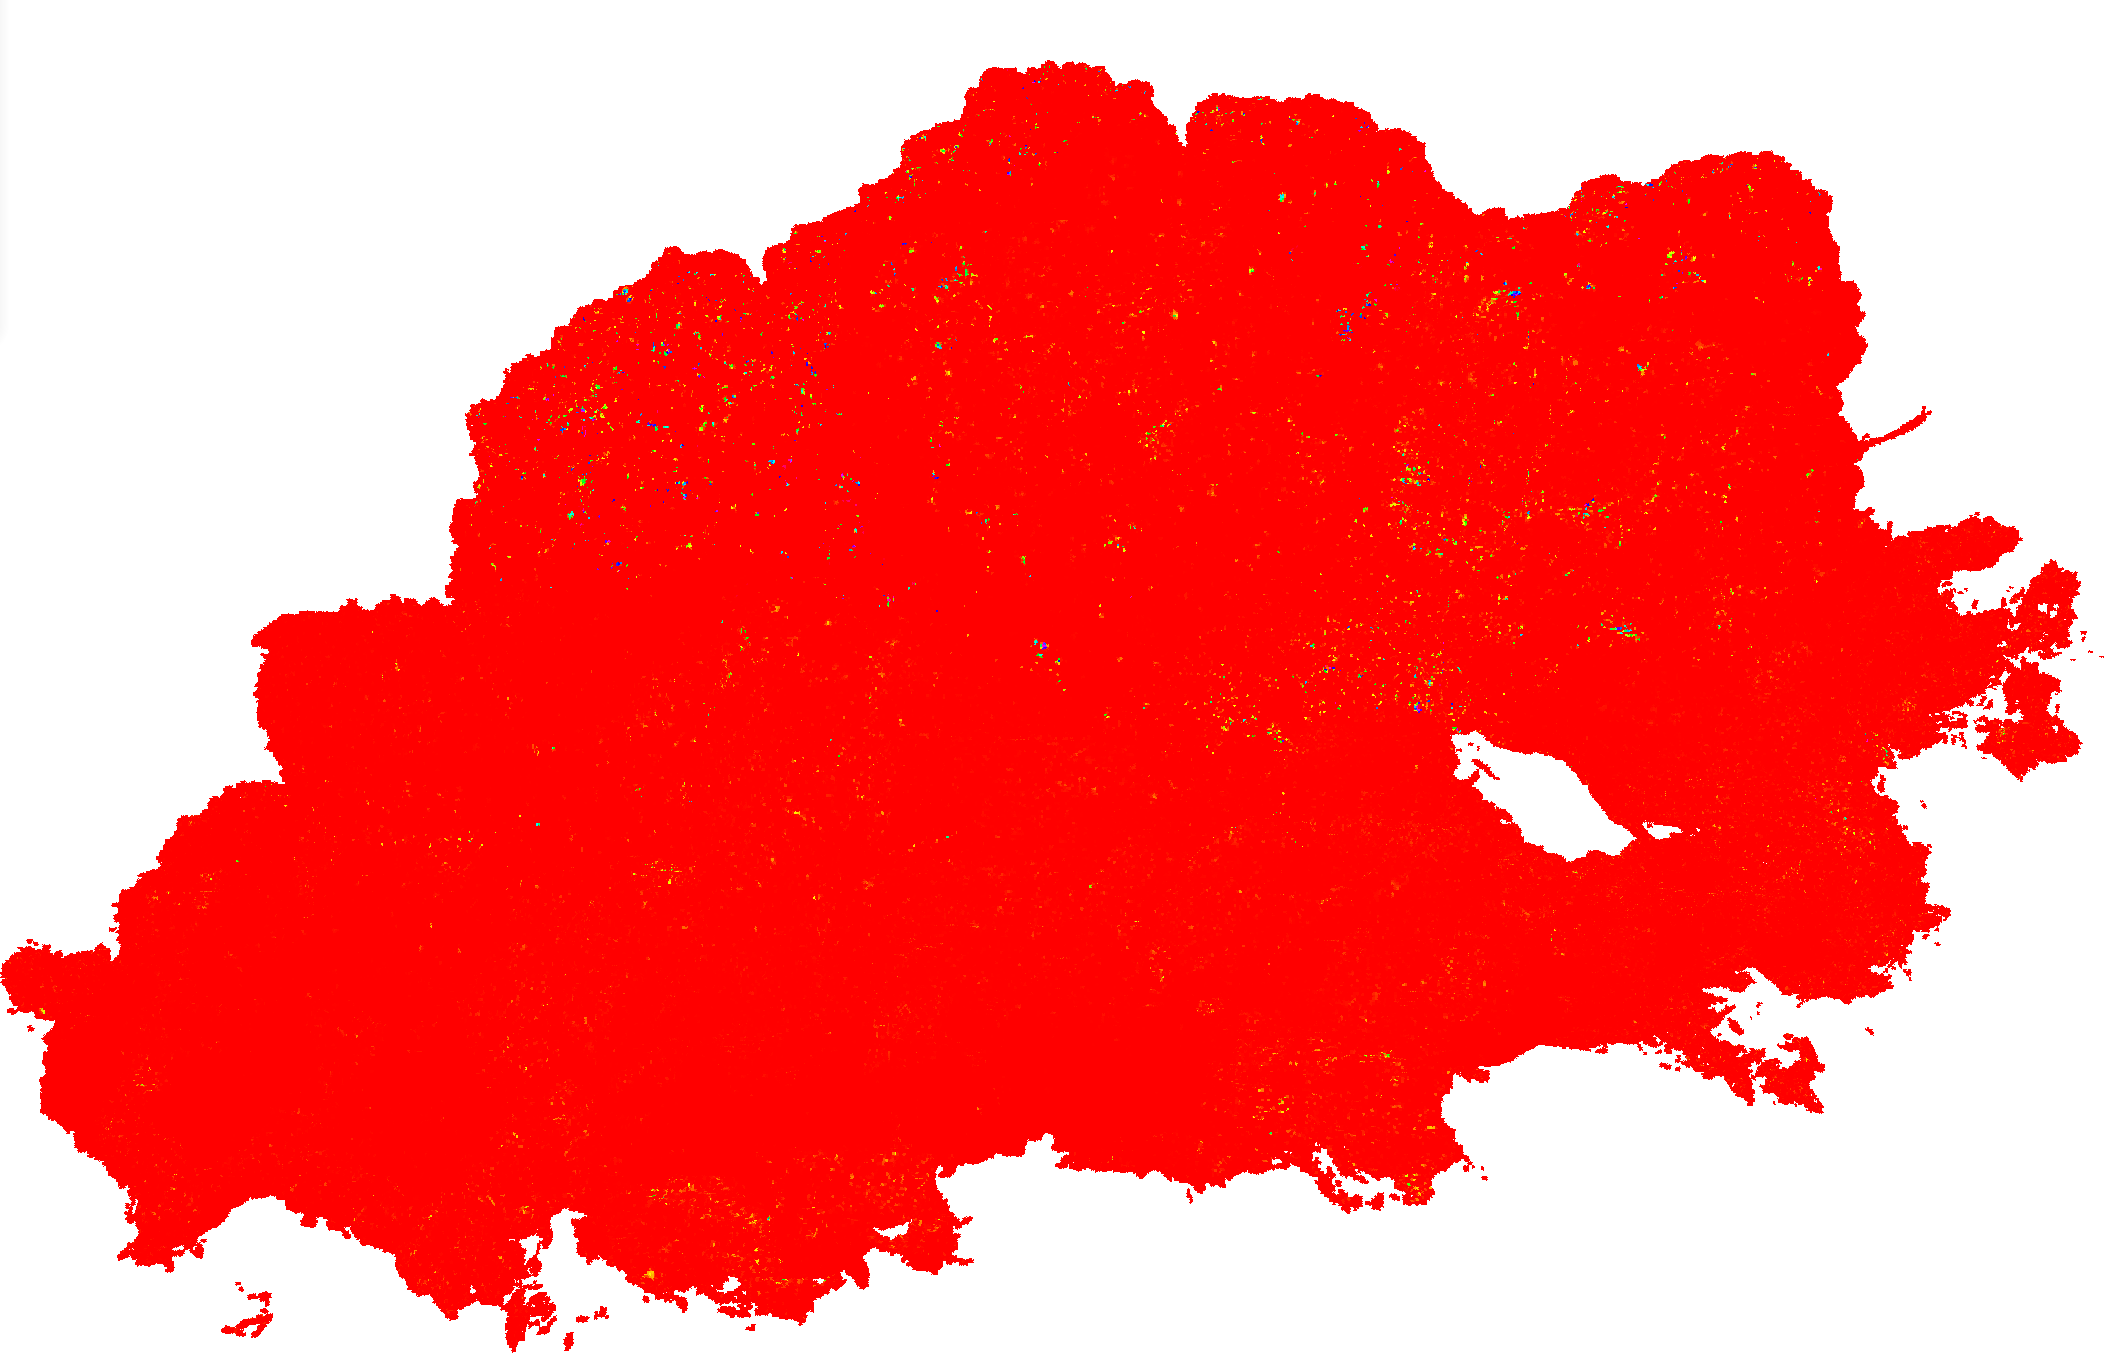
\includegraphics[width=0.45\textwidth]{figures/disney_cloud_half_res_first_temp.png}
    }
    \caption{Some shading options of the VDB viewer application. The exact color values do not matter in this example, these figures exist to illustrate general patterns. All renders are done using the half-resolution version of the Disney cloud \cite{DisneyCloud}. } \label{implementation:vdb_viewer:debug_views}
\end{figure}